\chapter{Phase 2: System Interaktion und Bedienung}

\section{User Stories}

Nun werden die Usecases aus Phase 1 mithilfe von User Stories weiter beschrieben. Dabei liegt der Fokus auf Szenarien, die eine Interaktion mit dem Smartwatch-System abbilden.
Die ersten beiden User Stories beschreiben zunächst einen typischen Hauptanwendungsfall der Uhr: Das Annehmen/Ablehnen/Tätigen von Anrufen von dem verbundenen Smartphone.
Um dem Produkt eine detailgetreue Anleitung für einen reibungslosen Einrichtungsprozess beizulegen, wurde eine User Story speziell für das Einrichten, bzw. Koppeln der Smartwatch mit einem Smartphone definiert.
Da eine Kernfunktionion der Smartwatch darin besteht, sie für Fitness-Tracking verschiedener sportlichen Aktivitäten einzusetzen, wurden mehrere User Stories für diese Anwendungsfälle entworfen. Im folgenden wird die User Story "Joggen gehen" beschrieben, weitere Fitness-User Stories finden sich im Anhang an diese Arbeit.
\begin{figure}[H]
\centering\
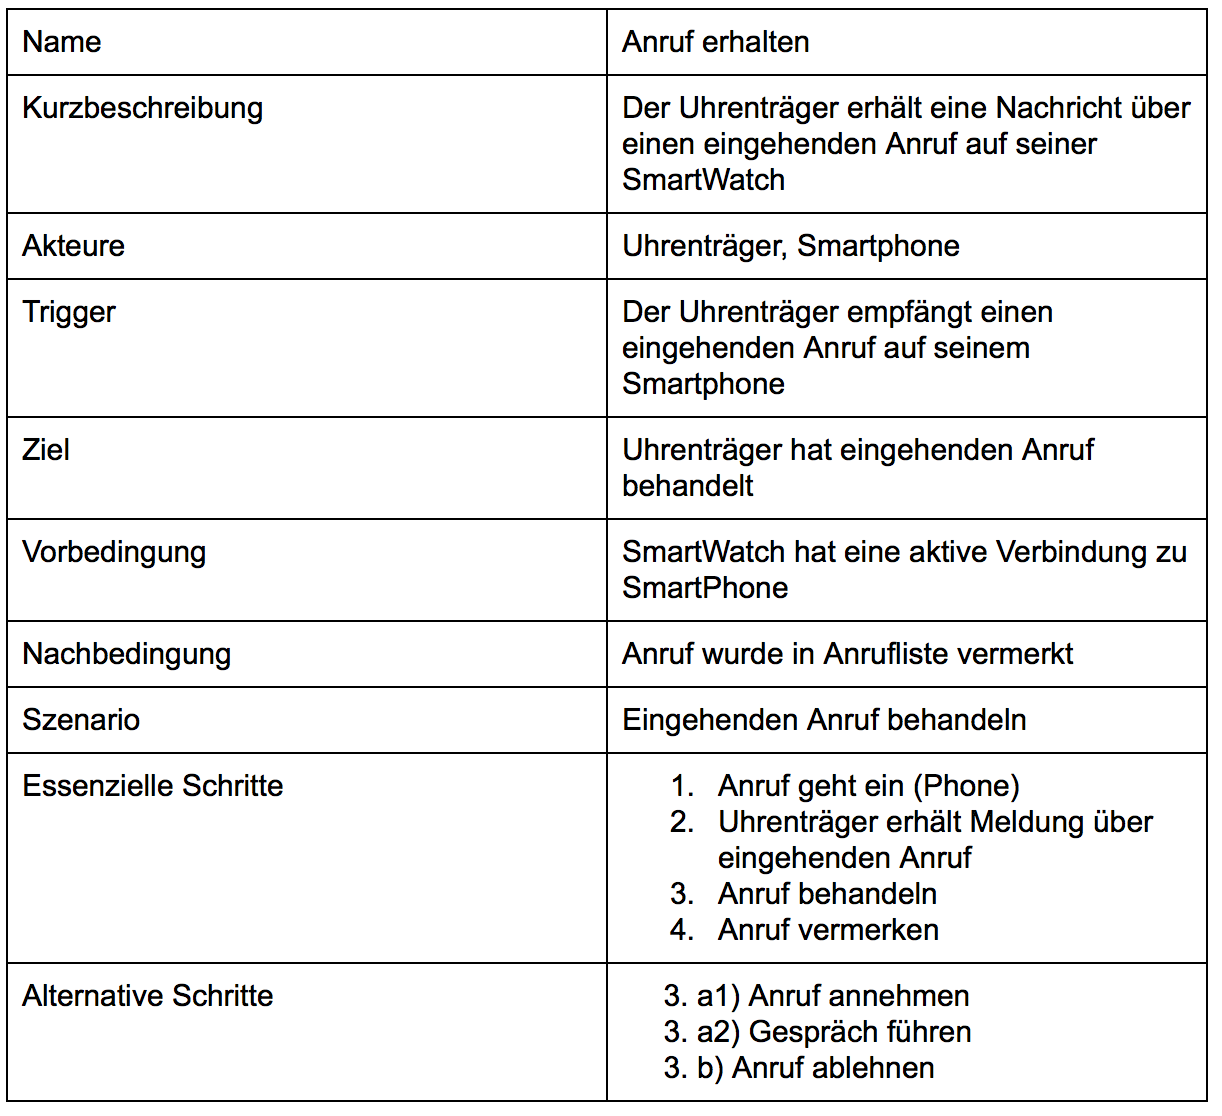
\includegraphics[width=10cm]{img/story_in}
\caption{User Story - Eingehender Anruf}\label{fig:story-in}
\end{figure}
\begin{figure}[H]
\centering\
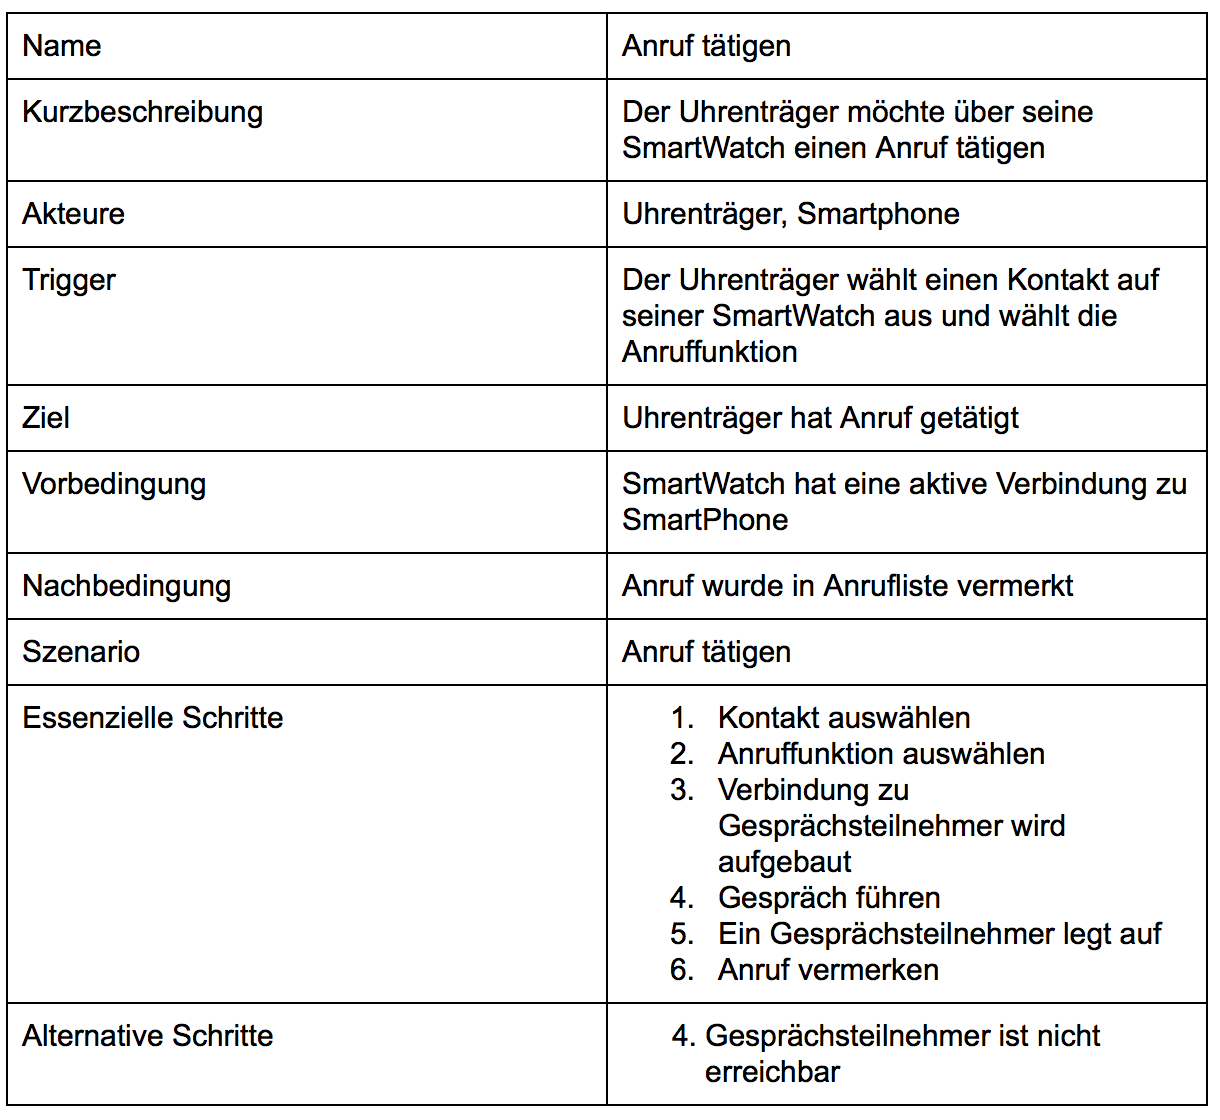
\includegraphics[width=10cm]{img/story_out}
\caption{User Story - Anruf tätigen}\label{fig:story-out}
\end{figure}
\begin{figure}[H]
\centering\
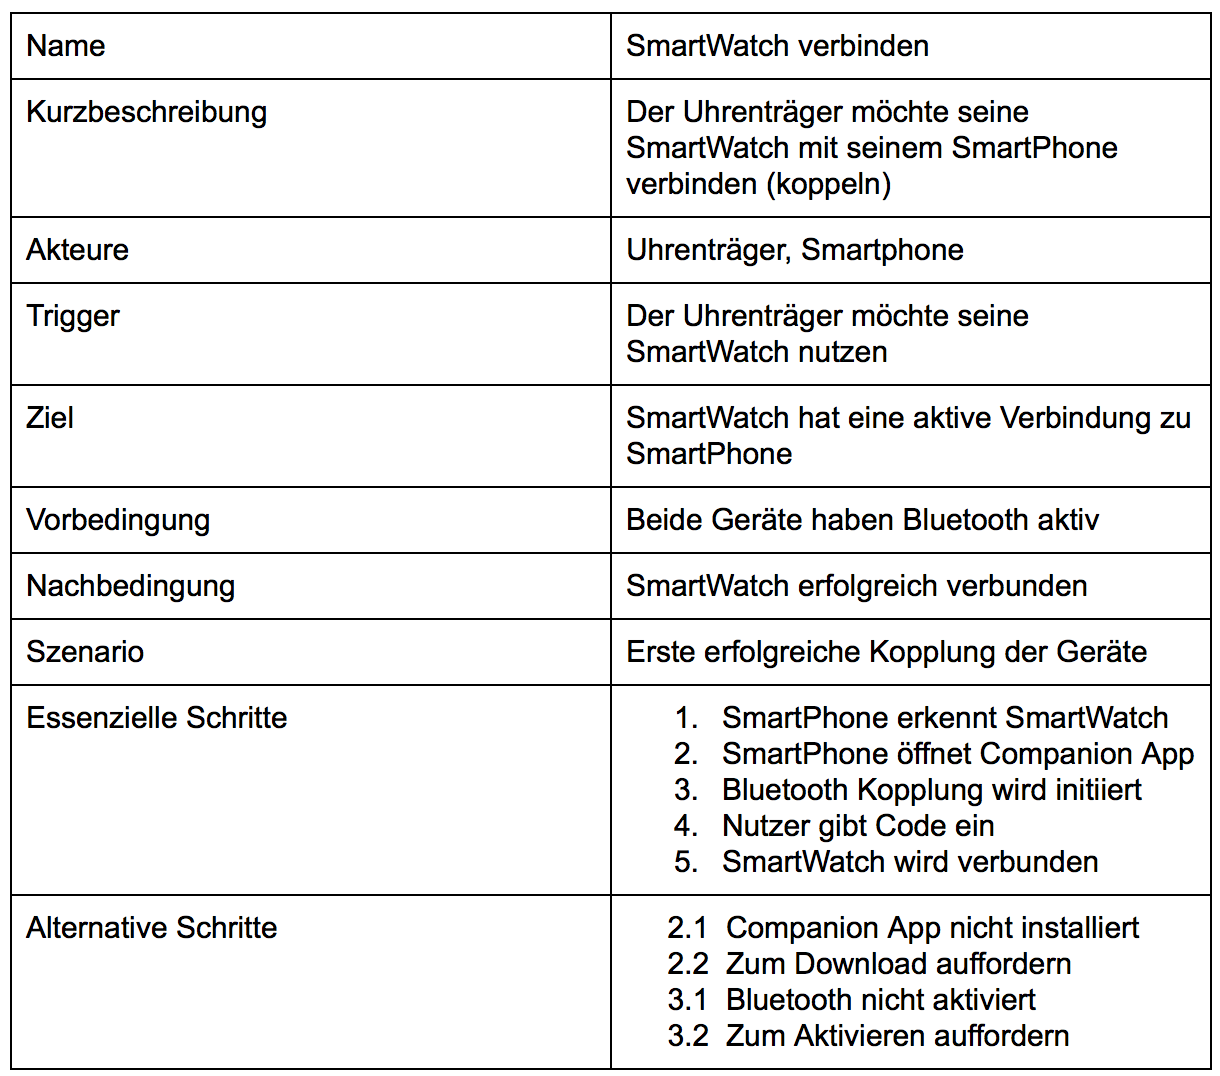
\includegraphics[width=10cm]{img/story_pairing}
\caption{User Story - Pairing}\label{fig:story-pairing}
\end{figure}
\begin{figure}[H]
\centering\
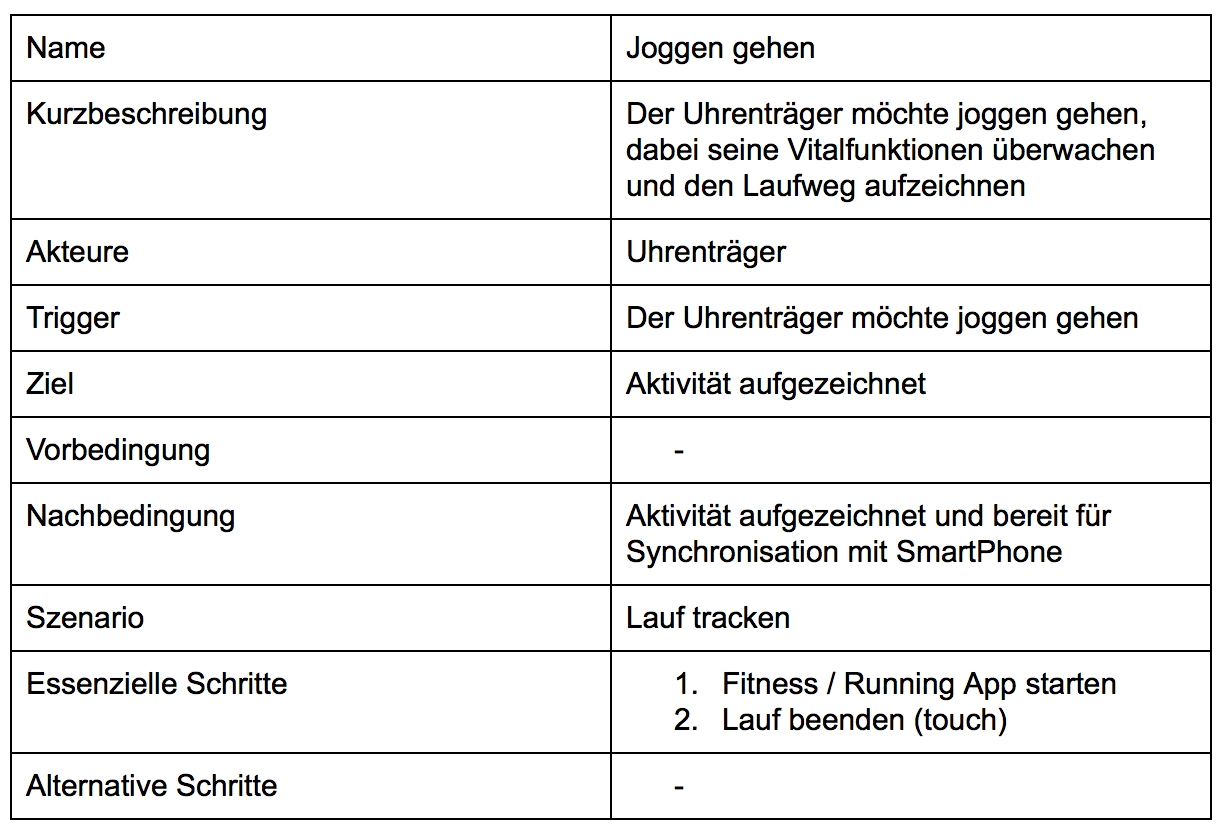
\includegraphics[width=10cm]{img/story_joggen}
\caption{User Story - Fitness}\label{fig:story-joggen}
\end{figure}

\section{Sequence Diagram}

\section{State Diagram}

\section{Timing Diagram}

